\section{MATLAB environment}
	As mentioned on chapter \textbf{\ref{ch:setup}}, FLIR software provides as output variables indexed matrices in .mat format, which is MATLAB variable format. Each pixel contains temperature information about itself, it is possible to visualize an example on a scaled image on the following figure:

	\begin{figure}[H]
		\centering
		\captionsetup{justification=centering}
		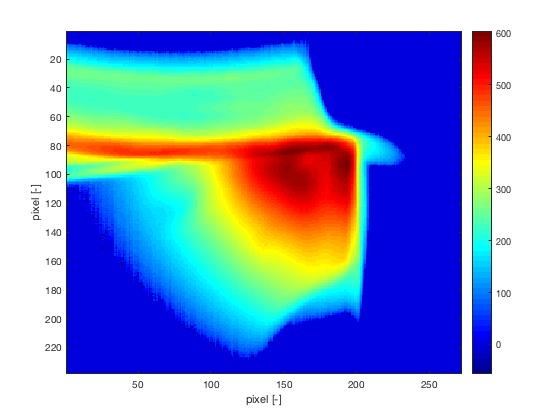
\includegraphics[width=0.9\linewidth]{Cap4/TempDist.jpg}
		\caption{Scaled image showing temperature distribution}
		\label{fig:tempdist}
	\end{figure}

	From figure \textbf{\ref{fig:tempdist}} with MATLAB Image Processing Toolbox support it possible to extract many informations about the image, such as:

	\begin{itemize}
		\item Edges recognition
		\item Image segmentation for tool, chip and workpiece
		\item Detection of tool tip
		\item Determine isotherms along tool
	\end{itemize}
	
\section{Auxiliar functions}
	\subsection{Contour plot}
	This is an important tool for this paper, contour plot is able to provide same level curves. Since the variable used on the process is a temperature matrix, this tool will calculate continuous lines, whose each pixel has a very close temperature measurements. Doing it with a determined and small tolerance, the lines calculated are isotherms of the image. Then, with these lines it is also possible to get its coordinates, which it will be essential to calculate heat carried away from volume control by means of tool.

	\begin{figure}[H]
		\centering
		\captionsetup{justification=centering}
		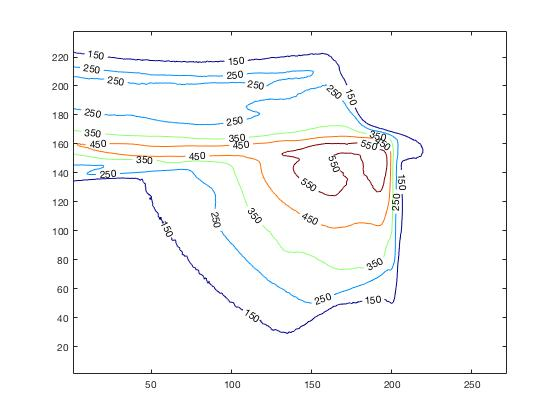
\includegraphics[width=0.6\linewidth]{Cap4/contour.jpg}
		\caption{Contour plot}
		\label{fig:contour}
	\end{figure}

	\subsection{Hough lines transformation}
	Hough transform is a extensively method used in computer vision. It is a extraction feature for complex geometries, using normal parametrization for straight lines \cite{duda1972use}. Concerning about the images, the rake and clearance face can be mapped by means of hough lines transformation in MATLAB. It is necessary to provide a probable angle range in what the angular coefficient of seeked lines are defined. More precise is this angle range, more reliable and faster will be the output.

	The test bench, where the experiments were held, allows a fixed placement of tool.

	\begin{figure}[H]
		\centering
		\captionsetup{justification=centering}
		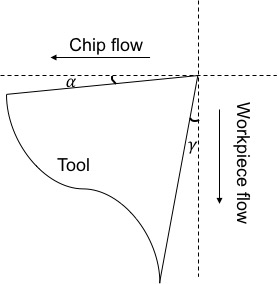
\includegraphics[width=0.4\linewidth]{Cap4/imgset.jpg}
		\caption{Placement of tool}
		\label{fig:imgset}
	\end{figure}

	It means the angle between the rake face and horizontal line and the angle between clearance face and vertical line are always the designed rake and clearance angles, respectively. In other words, the tool does not rotate in relation to the reference axes. Because of this, it is possible to peform hough transformation on the image, being very accurate. As the rake and clearance angle are always $6^{o}$ and $3^{o}$, respectively, the hough transform processing will last a shoter time with predetermined angles than otherwise.

\section{Implementation steps}
	\subsection{Overview}	

	The final aim of the program was be able to identify the tool and chip shapes, then the analysis could extract and provide features that were essential for the results of this paper. By means of image processing and some input data, features like maximum cutting zone temperature, maximum chip temperature, heat flows through chip and tool are some examples of what the code is able to provide.	

	FAZER tabela COM INPUT/OUTPUT
	\subsection{Finding tool edges}

		fazendo teste para ser detectado no github.fhdjskfhjdkfhjdskgfHJDGhfj

		\subsubsection{Rake and clearance face}

		\subsubsection{Tool tip coordinates}

	\subsection{Maximum temperatures}

	\subsection{Temperature fields}

	\subsection{Heat flows - Chip and Tool}

		\subsubsection{Heat partitions}

	
	
% 	\begin{mdframed}[backgroundcolor=lightgray!25!]
% 		\begin{alltt}\fontsize{9pt}{8pt}\fontfamily{pcr}\selectfont
% N.degree:  integer representing the degree of the functions.
% N.knots:   n x 2 matrix, with the knot intervals where the function is non-zero,
%            where n is the number of intervals, the first column has the start of
%            the interval and the second column has the end of it.
% N.coefs:   n x (p+1) matrix, with the coefficients of the polynomial for that
%            given interval. The first column contains the coefficient for the
%            p-th power, and the last column contains the constant.
% 		\end{alltt}
% 	\end{mdframed}